\chapter{Reference Framework} % Chapter title
\label{ch:referenceFramework} % For referencing the chapter elsewhere, use \autoref{ch:examples} 

%----------------------------------------------------------------------------------------
%-------------------------------------------------------------------------
\section{Theoretical Framework}

\subsection{\ac{GUR} and \ac{PX}}
\label{subsec:gur}
According to \textcite{macklin2016games} a game is a work made to express, impart and provide experiences, producing play when interacting with it. \textcite{rogers2014level} defines a game as an activity that requires at least a player, has rules and a victory condition. \textcite{koster2013theory} states that a game is an iconic representation of real world patterns. \textcite{schell2015art} considers a game as a problem solving activity, which is approached with a playful attitude. Games create an imaginary world that absorbs players' full attention \autocite{michael:2006}. The main goal of games is to provide a fun and engaging experience to players \autocite{Moosajee,Zammitto2014}. Thus, evaluating the quality of the experience the games provide to players.

\ac{PX} is one of the most significant factors in determining the success of digital games in terms of aspects such as fun, flow, enjoyment, engagement, satisfaction, pleasure and playability. However, this concept is not used consistently in the literature \autocite{Wiemeyer2016} and sometimes is used interchangeably with other concepts such as playability, gamer experience, game experience or \ac{UX} \autocite{Bernhaupt2015}. For instance, in \autocite{Chu2011,GonzalezSanchez2009}, \ac{PX} is considered to be described by playability, while in \autocite{Nacke2009} playability is considered to be a prerequisite for a high quality of \ac{PX}. An accepted definition of \emph{\ac{PX}} is that it can be considered as an extension of \ac{UX} \autocite{Wiemeyer2016,GonzalezSanchez2009,Bernhaupt2015}. While, \ac{UX} represents the quality of interaction between users and software \autocite{Wiemeyer2016,Bernhaupt2015,Calvillo-Gamez2015}; while \ac{PX} denotes the personal experience of playing digital games, thus it involves subjective perceptions of players \autocite{Wiemeyer2016,Chu2011}. The goal of evaluating \ac{PX} is to improve interaction between players and games.

\ac{GUR} consists in the observation and analysis of \ac{PX} applying methods from different fields such as usability, psychology, play testing \autocite{Wiemeyer2016}, gameplay metrics \autocite{Drachen2013} and physiological evaluation \autocite{Nacke2015}. Thus, \ac{GUR} enables and fosters collaboration between \ac{PX} professionals, game developers and academic researchers \autocite{desurvire_methods_2013}. Below, \ac{GUR} methods and considerations when evaluating digital games are presented.

%Existing \ac{GUR} methods can be employed for evaluating \ac{PX}, however they may need adaptations for rehabilitation exergames since there are some issues which may alter \ac{PX} during interaction. These issues include: (i) exergames use non traditional interaction devices, such as movement sensors; (ii) players impairment may impose limitations to interaction, and (iii) intervention of other people (e.g. therapists) may be required \autocite{Wiemeyer2015,Nijholt2008}. Consequently, these issues should be considered when performing a \ac{PX} evaluation.

\subsection{\ac{GUR} Evaluation Aspects}
\label{subsec:aspects}

Selecting the aspects to be evaluated is a crucial task to be overcome when preparing an evaluation. However, selecting the most important aspects to evaluate is difficult \autocite{Nacked}. This selection depends on factors such as evaluation goal, available resources and development maturity of the evaluated game. There are different approaches to evaluate \ac{PX} in a general way, \textcite{Sanchez2009} presents an approach to evaluate \ac{PX} through playability; meanwhile, \textcite{Calvillo-Gamez2015} present a selection of aspects known as \emph{Core Elements of the Gaming Experience}, which are necessary but not sufficient for games to provide a positive experience.

Motivation and willingness to play can be evaluated in terms of other aspects such as immersion \autocite{Lapas2015,Nacke2009,VandenAbeele2016,Wiemeyer2016,Nijhar2012,Sanchez2009,Desurvire2009,Nijholt2008}, enjoyment \autocite{Ho2017,Li2016,VandenAbeele2016,Zhao2016,Li2006,Berkovsky2010}, challenge \autocite{Moosajee,Nacke2009,VandenAbeele2016,Wiemeyer2016,Desurvire2009}, flow \autocite{Lapas2015,Bernhaupt2015,Nacke2009,Wiemeyer2016,Nijholt2008}, presence \autocite{Lapas2015,Mader2012,Ho2017,Wiemeyer2016}, 
emotion \autocite{Bernhaupt2015,Sanchez2009,Wiemeyer2016}, engagement \autocite{Yanez-Gomez2017,Wiemeyer2016}, negative-positive affect \autocite{Nacke2009}, interest \autocite{VandenAbeele2016}, preference \autocite{Zhao2016}, autonomy \autocite{Wiemeyer2016,VandenAbeele2016} and 
absorption \autocite{Lapas2015}. Meanwhile, playability or usability, can be evaluated through aspects like satisfaction \autocite{Yanez-Gomez2017,Zhao2016,Sanchez2009}, ease of use \autocite{Moosajee,VandenAbeele2016,Cameirao2010}, learnability \autocite{GonzalezSanchez2009,Desurvire2009} and
acceptance \autocite{Yanez-Gomez2017}. Finally, game design can be evaluated using aspects including story \autocite{Moosajee,Desurvire2009}, clarity of goals \autocite{VandenAbeele2016,Desurvire2009}, tension, competence \autocite{Wiemeyer2016,Nacke2009}, camera \autocite{Moosajee},
game pace \autocite{Moosajee,Desurvire2009}, aesthetics, stimulation, identification \autocite{Bernhaupt2015}, audiovisual appeal, meaning \autocite{VandenAbeele2016}, involvement, curiosity, fantasy \autocite{Wiemeyer2016}, game adaptation \autocite{Wiemeyer2015,Ni2014,Cameirao2010,Nijholt2008} and social play \autocite{Wiemeyer2015,Sanchez2009,Yanez-Gomez2017,Lapas2015}.

However, as shown in \autoref{tab:aspects}, \ac{GUR} aspects are categorised inconsistently within the literature. Aspects are categorised as properties, components, dimensions, constructs, facets, factors, areas or parameters.

\begin{table}[bht]
\caption{Categorisation inconsistencies for \ac{PX} evaluation aspects}
\label{tab:aspects}
\myfloatalign
\resizebox{0.7\linewidth}{!}{
\begin{tabular}{p{5.5em}lllllllllll}
\toprule
\multirow{2}{*}{\spacedlowsmallcaps{Aspect}} & \multicolumn{11}{c}{\spacedlowsmallcaps{Referred as}} \\
\cline{2-12}
&\rot{\small{\textit{Playability Aspect} \autocite{Yanez-Gomez2017}}}
&\rot{\small{\textit{Playability Property} \autocite{Sanchez2009}}}
&\rot{\small{\textit{GX Component} \autocite{Nijhar2012}}}
&\rot{\small{\textit{\ac{PX} Element} \autocite{Wiemeyer2016}}}
&\rot{\small{\textit{\ac{UX} Dimension} \autocite{Bernhaupt2015}}}
&\rot{\small{\textit{\ac{PX} Dimension} \autocite{Nacke2009}}}
&\rot{\small{\textit{\ac{PX} Component} \autocite{VandenAbeele2016}}}
&\rot{\small{\textit{\ac{UX} Facet} \autocite{Lapas2015}}}
&\rot{\small{\textit{Factor} \autocite{Ho2017}}}
&\rot{\small{\textit{Area} \autocite{Moosajee}}}
&\rot{\small{\textit{Gameplay Parameter} \autocite{Zhao2016}}} \\
\midrule
Immersion &  & X & X & X &  & X & X & X &  &  & \\
\midrule
Enjoyment &  &  &  &  &  &  & X &  & X &  & X \\
\midrule
Challenge &  &  &  & X &  & X & X &  &  & X & \\
\midrule
Flow &  &  &  & X & X & X &  & X &  &  & \\
\midrule
Presence &  &  &  & X &  &  &  & X &  &  & \\
\midrule
Social play & X & X &  & X &  &  &  & X &  &  & \\
\midrule
Satisfaction & X & X &  &  &  &  &  &  &  &  & X \\
\midrule
Feedback &  &  &  & X &  &  & X &  &  &  & \\
\midrule
Ease of use &  &  &  &  &  &  & X &  &  & X & \\
\midrule
Emotion &  & X &  & X & X &  &  &  &  &  & \\
\midrule
Engagement & X &  &  & X &  &  &  &  &  &  & \\
\bottomrule
\end{tabular}}
\end{table}

\subsection{\ac{GUR} Evaluation Methods}
\label{subsec:methods}
The goal of applying \ac{GUR} methods is to determine whether a game offers a compelling and engaging experience to players \autocite{Yanez-Gomez2017,Bernhaupt2015}, collecting \ac{PX} data before, during and/or after players interact with the game (or game prototype) \autocite{Wiemeyer2016,Nacke2015,Mueller2015,Drachen2013}. Also, \ac{UX} and usability methods are commonly used for evaluating \ac{PX} \autocite{Yanez-Gomez2017,McAllister2015}. However, these are not sufficient for evaluating games, since standard metrics, such as task completion or error rates, do not map to metrics that may assess \ac{PX} properly. Therefore, traditional usability metrics should be used along with other forms of evaluation or should be extended \autocite{Wiemeyer2016,McAllister2015,Bernhaupt2015,Nackea,Hoysniemi2006}. \autoref{tab:methods} presents an overview of available \ac{GUR} methods for evaluating \ac{PX} grouped into five categories. Those categories are detailed below.

\begin{table}[bth]
\caption[\ac{GUR} methods for \ac{PX} evaluation]{\ac{GUR} methods for \ac{PX} evaluation}
\label{tab:methods}
\myfloatalign
\resizebox{0.86\linewidth}{!}{
\begin{tabular}{p{2.5cm}p{3.5cm}l}
\toprule
%----------------------
\spacedlowsmallcaps{Category} 
& \spacedlowsmallcaps{Description}
& \spacedlowsmallcaps{Method}
\\ \midrule
%----------------------
\multirow{12}{2.5cm}{User-oriented}
&
\multirow{12}{3.5cm}{Evaluation data is collected from players who represent the target audience}
&
Questionnaire \autocite{Yanez-Gomez2017,Ho2017,Wiemeyer2016,Nacke2015,Mueller2015,Zhao2016,Lapas2015,Nijhar2012,Nackea}
\\
&&
Interview \autocite{Wiemeyer2016,Moosajee,Nacke2015,Nijhar2012,Nackea}
\\
&&
Video recording \autocite{Wiemeyer2016,Moosajee,Mueller2015,Nijhar2012}
\\
&&
Field-Behavioural observation \autocite{Yanez-Gomez2017,Wiemeyer2016,Nacke2015}
\\
&&
Think-aloud protocol \autocite{Wiemeyer2016,Nacke2015,desurvire_methods_2013}
\\
&&
Focus groups \autocite{Yanez-Gomez2017,Nacke2015}
\\
&&
\ac{RITE} \autocite{Moosajee,Nackea}
\\
&&
Co-discovery learning \autocite{Yanez-Gomez2017}
\\
&&
Question-asking protocol \autocite{Yanez-Gomez2017}
\\
&&
Peer tutoring \autocite{Hoysniemi2003}
\\
&&
Prisoner dilemma task \autocite{Mueller2015}
\\
&&
Ethnography \autocite{Nackea}
\\\midrule
%----------------------
\multirow{4}{2.5cm}{Expert-oriented}
&
\multirow{4}{3.5cm}{A group of experts plays the role of players and inspect games}
&
Heuristic evaluation \autocite{Yanez-Gomez2017,Wiemeyer2016,Nacke2015,desurvire_methods_2013,Nackea,Nacke2009,Desurvire2009,Federoff2002}
\\
&&
Guidelines or standard inspections \autocite{Yanez-Gomez2017}
\\
&&
Cognitive walk through \autocite{Yanez-Gomez2017}
\\
&&
Pluralistic walk through \autocite{Yanez-Gomez2017}
\\\midrule
%----------------------
\multirow{3}{2.5cm}{Automated}
&
\multirow{3}{3.5cm}{Evaluation data is collected direct from games}
&
Gameplay metrics \autocite{Nacke2015,Nackea,Nacke2009}
\\
&&
Game logs \autocite{Wiemeyer2016}
\\
&&
A/B Testing \autocite{desurvire_methods_2013}
\\\midrule
%----------------------
\multirow{7}{2.5cm}{Physiological}
&
\multirow{7}{3.5cm}{Evaluation data is collected direct from players' body surface}
&
Biometrics analyse \autocite{Nacke2009}
\\
&&
\ac{EEG} \autocite{Wiemeyer2016,Nacke2015}
\\
&&
\ac{EMG} \autocite{Wiemeyer2016,Nacke2015}
\\
&&
\ac{EDA} \autocite{Wiemeyer2016,Nacke2015}
\\
&&
\ac{HR} \autocite{Wiemeyer2016,Nacke2015}
\\
&&
Body movement coding \autocite{Mueller2015,Nijhar2012}
\\
&&
Eye-tracking \autocite{Wiemeyer2016,Nackea}
\\\midrule
%----------------------
\multirow{3}{2.5cm}{Psychological}
&
\multirow{3}{3.5cm}{The collected data is used to model player and \ac{PX}}
&
Persona modelling \autocite{Wiemeyer2016,Nackea}
\\
&&
Player modelling \autocite{Wiemeyer2016,Nackea}
\\
&&
Cultural debugging \autocite{Nackea}
\\
%----------------------
\bottomrule
\end{tabular}}
\end{table}

\subsubsection{User-oriented}
User-oriented methods involve players during \ac{PX} evaluations to gather data such as behaviours, reactions, opinions, comments and suggestions \autocite{Yanez-Gomez2017,Bernhaupt2015,Drachen2013}. Frequently used methods include questionnaires \autocite{Yanez-Gomez2017,Ho2017,Wiemeyer2016,Nacke2015,Mueller2015,Bernhaupt2015,Zhao2016,Lapas2015,Nijhar2012,Nackea}, interviews \autocite{Wiemeyer2016,Moosajee,Nacke2015,Nijhar2012,Nackea}, video recording \autocite{Wiemeyer2016,Moosajee,Mueller2015,Nijhar2012}, field observation \autocite{Yanez-Gomez2017,Wiemeyer2016,Nacke2015}, think-aloud protocol \autocite{Wiemeyer2016,Nacke2015,desurvire_methods_2013}, focus groups \autocite{Yanez-Gomez2017,Nacke2015}, co-discovering learning \autocite{Yanez-Gomez2017}, question-asking protocol \autocite{Yanez-Gomez2017} and ethnography \autocite{Nackea}. Although, there are some standardised questionnaires and scales which can be used \autocite{denisova_convergence_2016,VandenAbeele2016,Calvillo-Gamez2015,Brockmyer2009,Poels2008,DeKort2007,Vorderer2004}, the use of ad-hoc questionnaires is the most preferred approach \autocite{Yanez-Gomez2017}. Some user-oriented methods, such as \ac{RITE} \autocite{Moosajee,Nackea}, have been developed in the game development context. Also, evaluators may need adapt or create methods to meet specific evaluation requirements. For instance, evaluators have employed peer tutoring for evaluating \ac{PX} in exergames for children \autocite{Hoysniemi2003}; and prisoner dilemma task for evaluating players competitiveness and cooperation behaviours in an exergame \autocite{Mueller2015}.

User-oriented methods can be used along the whole development life-cycle based on the current needs and the availability of users to participate. If the number of available users is low, methods such as interviews, field observations, think-aloud protocol and co-discovery learning are convenient. In case of questionnaires, focus groups and \ac{RITE} evaluators should consider some issues. First, evaluators should plan well in advance if a high number of users is needed for a questionnaire evaluation. In such a case, they should plan a recruitment strategy. Similarly, evaluators should determine the number of sessions to be conducted when using focus groups. Finally, \ac{RITE} requires evaluators and developers to test and fix the evaluated game iteratively during an evaluation session. In that case, evaluators should adapt evaluation location to facilitate conditions for developers to fix identified issues.

\subsubsection{Expert-oriented}
In this case, a group of experts inspect a game to identify possible issues which may affect \ac{PX} \autocite{Bernhaupt2015,Yanez-Gomez2017}. There are two common approaches when applying expert-oriented methods: experts assess whether a game meets a set of principles; i.e., heuristics \autocite{Yanez-Gomez2017,Wiemeyer2016,Nacke2015,desurvire_methods_2013,Nackea,Nacke2009,Desurvire2009,Federoff2002}, guidelines or standards \autocite{Yanez-Gomez2017}; and experts play the role of a player performing a set of typical tasks, using cognitive and/or pluralistic walk-through \autocite{Yanez-Gomez2017}.

The most used expert-oriented methods are heuristic evaluation \autocite{Desurvire2009,Federoff2002,Hochleitner2015,Tondello2016} and guidelines inspection \autocite{Yanez-Gomez2017}, which are convenient for evaluating games when players are not available. In the case of exergames, there are some guidelines \autocite{Wiemeyer2015,Pasch2009,Isbister2015,Mueller2014} that evaluators can use. Expert-oriented methods are appropriate for performing \ac{PX} evaluations during early stages of game development \autocite{Bernhaupt2015,McAllister2015,desurvire_methods_2013}. However, results of these methods depend directly on evaluators’ expertise. 

\subsubsection{Automated}
Automated methods allow collecting \ac{PX} data from games using programmed hooks \autocite{Nacke2015}. The collected data will be used to get information about players behaviour during interaction. Automated evaluation methods are considered objective since they allow collecting quantitative data. Additionally, automated methods can be useful for performing A/B testing, which is used to compare several versions of a game and decide over different design alternatives \autocite{desurvire_methods_2013}. The most common automated methods are game-play metrics \autocite{Nacke2015} and game logs \autocite{Drachen2013,Wiemeyer2016}.

\subsubsection{Physiological}
These methods allow collecting player’s body signals, which are used to understand the experience that players have while interacting with a game \autocite{Wiemeyer2016,Nacke2015}. Evaluators can use these methods to monitor internal body reactions before, during and after interaction \autocite{Mueller2011}. Physiological methods include eye-tracking \autocite{Wiemeyer2016,Nackea}, \ac{EDA} \autocite{Wiemeyer2016,Nacke2015}, \ac{EMG} \autocite{Wiemeyer2016,Nacke2015}, \ac{EEG} \autocite{Wiemeyer2016,Nacke2015} and \ac{HR} \autocite{Wiemeyer2016,Nacke2015}. Like automated, physiological methods are objective. Also, biometric analyse \autocite{Nacke2009} or body movement coding \autocite{Mueller2015,Nijhar2012} can be used to analyse the data collected during an evaluation. In case of exergames, evaluators should be careful when using \ac{EDA}, \ac{EMG} or \ac{EEG} measurement since patient’s movements could be limited by data collection instruments, which is a difficulty if an exergame requires movements like shifts or squats.

\subsubsection{Psychological}
Psychological methods are useful for collecting data about cognitive, perceptual and emotional experiences \autocite{Wiemeyer2016,Nackea}. Those data are relevant since perceived experience is a personal and subjective perception. A well-known psychological method is Persona modelling \autocite{Wiemeyer2016,Nackea}, which allows representing and understanding players mental model. Player modelling is a method used to adapt \ac{PX} according to players behaviour during gameplay \autocite{Wiemeyer2016,Nackea}. Cultural debugging is used to determine cultural differences that may affect \ac{PX} \autocite{Nackea}. Psychological methods are useful to identify target users who can participate in evaluations.

%\subsubsection{Evaluation Methods for Rehabilitation Exergames}

%In the case of rehabilitation exergames, all the above mentioned methods can be employed to evaluate \ac{PX}. However, some issues that may affect \ac{PX} and rehabilitation process should be considered. These issues include: 

%\begin{itemize}
    %\item Evaluation should not only focus on fun, but also on the health goal that is being pursued by a game \autocite{Iacovides2015}.
    %\item Game should adapt to particular player's needs \autocite{Wiemeyer2015,Ni2014,Cameirao2010,Nijholt2008}.
    %\item Player modelling should consider target audience's health conditions \autocite{Mader2012,Wiemeyer2015}.
    %\item Cheating the rehabilitation goal of a game should be avoided \autocite{Ni2014}.
    %\item Player distractions should be avoided \autocite{Ni2014}.
    %\item Family members and clinicians should be included since they may intervene during interaction \autocite{Wiemeyer2015}.
    %\item Game feedback should be evaluated, since it has to be positive \autocite{Wiemeyer2015}.
%\end{itemize}

In the case of digital games used in physical rehabilitation, there is no a defined approach to evaluate \ac{PX}. Some authors state that methods have to be selected, adapted and/or combined depending on the particular case being evaluated \autocite{Yanez-Gomez2017,Wiemeyer2016,Mueller2015}. Additionally, an objective evaluation may be achieved collecting qualitative and quantitative data. That is known as mixed or multi-method approach \autocite{Nacke2009,Iacovides2015,Drachen2013,Mueller2015,Zammitto2014}.

\subsection{\ac{GUR} Evaluation Instruments}
\label{subsec:instruments}
The selection of tools to be used while evaluating \ac{PX} depends on the methods, aspects and game involved in the evaluation. Evaluators can use different standardised questionnaires to evaluate \ac{PX} depending on the aspects to be evaluated.

The \textit{\ac{PX} inventory} \autocite{VandenAbeele2016} is a scale based on the \ac{MDA} framework and evaluates eleven aspects of \ac{PX} including enjoyment, mastery, ease of control, progress feedback and audio-visual appeal. It groups the aspects into three levels: value, functional and psycho-social, and each level is evaluated using a sub-scale. The inventory was developed along two iterations, involving a group of experts and based on other 124 existing scales. 

\textit{\ac{CEGEQ}} \autocite{Calvillo-Gamez2015} is composed of 38 items and was developed involving game reviews and interviews with a game designer, two game reviewers and one player. The aspects evaluated by this questionnaire include: enjoyment, scenario, rules, ownership and control.

The \textit{\ac{GEQ}} is a modular questionnaire composed of a core questionnaire, a post-game questionnaire and social presence questionnaire \autocite{Poels2008}. This questionnaire was developed during focus groups and expert meetings considering existing questionnaires. Seven aspects are evaluated by the core questionnaire: sensory and imaginative immersion, tension, competence, flow, negative affect, positive affect and challenge.

The \textit{\ac{GEQ2}} \autocite{Brockmyer2009} is composed of 19 items and evaluate four aspects: absorption, flow, presence and immersion. It was developed along three iterations.

The \textit{EGameFlow Scale} \autocite{Fu2009} is composed of 42 items and allow evaluating concentration, goal clarity, feedback, challenge, autonomy, immersion, social interaction and knowledge improvement. This scale is intended to evaluate e-learning games; thus, an adaptation for evaluating other kinds of games may be required.

Furthermore, evaluators can use questionnaires for evaluating specific aspects. An immersion questionnaire is presented in \autocite{jennett2008measuring}, it allows evaluating immersion quantitatively based on basic attention, temporal dissociation, transportation, challenge, emotional involvement and enjoyment. Also, the \ac{SPGQ} \autocite{DeKort2007} evaluates social presence in terms of empathy, negative feelings and behavioural involvement. It was developed based on focus groups, interviews and another social presence scale. Additionally, \ac{UX} scales \autocite{Brooke1996} and questionnaires \autocite{Laugwitz2008,Hassenzahl2003,lund2001measuring} can be employed to evaluate aspects such as usability, ease of use and satisfaction.

With reference to expert-oriented methods, the heuristics presented in \autocite{Desurvire2009,Federoff2002,Tondello2016} can be employed for initial evaluations of game design. Similarly, there are design guidelines \autocite{Wiemeyer2015,Isbister2015,Mueller2014} and principles \autocite{Berkovsky2010} specialised for exergames. Regarding physiological methods, biometric storyboards \autocite{Mirza-Babaei2014} are appropriate to visualise, relate and analyse collected data; e.g., player's physiological data, self-reported events and in-game events.

Additionally, evaluators can use models to assess and validate \ac{PX} evaluation results. Some models include: the motivation model for exertion games \autocite{Li2016}, which is based on the \ac{SCT} and relates a game avatar with \ac{PX} in exergames. This model suggests that self-presence is positively associated with identification, which is also positively associated with enjoyment. Moreover, the presence, enjoyment and mood experience model \autocite{Ho2017} relates subjective level of presence, game enjoyment and mood experience to players' attitude towards exertion games. Furthermore, the model presented in \autocite{Mader2012} allows describing and analysing the relation among a player, a game and a therapy. This model assists in deciding which information should be collected, examining game design coherence and identifying constraints imposed by a therapy. Moreover, models such as the \ac{4LM} \autocite{Mueller2011}, the \ac{ISCAL} \autocite{Zhang2011} and the Dual Flow Model \autocite{Sinclair2007} may be useful to select which aspects are relevant to evaluate exergames.

Finally, \textcite{Ni2014} presents a design and evaluation framework for virtual rehabilitation based therapy games. The framework was developed with the active participation of a group of children and therapists. The authors present a list of design requirements for virtual rehabilitation based therapy games and characteristics of a game for health. \textcite{kendzierski1991physical} describe the physical activity enjoyment scale, which can be used to evaluate enjoyment in virtual rehabilitation based therapy games.

%----------------------------------------------------------------------------------------

\section{State of the Art}
\label{sec:px_ux_models}

To the extent of author's knowledge a \ac{PX} evaluation model for \acp{PREG} is not defined yet. However, some \ac{PX} models for general or specific purposes are presented below.

%----------------------
\subsection{The \ac{IMP}} 
% three elements: context,player and game
% time: pre-game, game, post-game

\textcite{Elson2014} present the \ac{IMP} which is an integrative model intended to be used for game user research purposes and is based on other literature. According to this model, \ac{PX} is comprised by three elements: player, i.e., (players' traits and states); game, i.e., the media and game characteristics and context, i.e. the setting and the social environment. The model claims that those three elements are affected along three consecutive phases. The model is illustrated in \autoref{fig:IMP_Model} and described below.

First, the Pregame phase corresponds to anything that occurs before playing a game. This phase results in the players' decision of playing or not a game. In this phase, the Context element is defined by cultural parameters that affect the player's selection of games. Context is characterised by some factors including cultural norms, marketing, social acceptance, peer groups and family. Meanwhile, the Player element is defined the characteristics of players as individuals, which includes biologic and demographic variables. Finally, the Game element is defined by its current availability and marketing attraction factors.

Second, the Game phase corresponds to the actual situation of playing or using a game. Context in this phase is determined by experimental aspects such as employed devices, location, platforms and the presence of other players. The Player element comprises the sum of psychological processes and behaviours including game enjoyment, presence and flow. The game element refers to the content and mechanisms of the game being played.

Third, the Post-Game phase includes the post-use effects of a singular or repeated episodes of game playing. The Post-Game forms a feedback loop that can affect the next gaming episode. In this phase, the Context element comprises all forms of communication caused or inspired by playing a game. The Player element is defined by internal states and behaviours of players after interacting with a game, which may be undesired. The effects on players can be short-term, i.e., temporary changes in thoughts, feelings and behaviours; or long-term, i.e., consequences of repeated episodes of game playing. The model does not describes the Game element in this phase.

\begin{figure}[bth]
\myfloatalign
{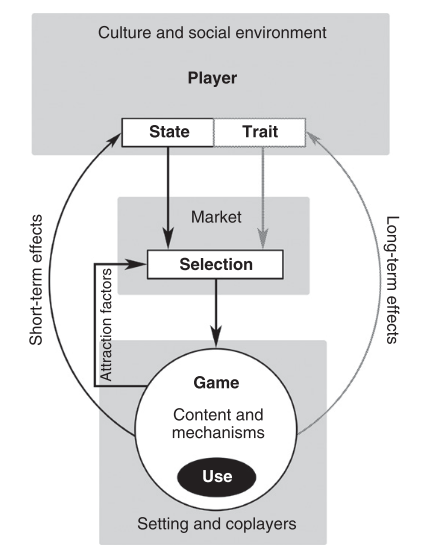
\includegraphics[width=.6\linewidth]{gfx/ref_framework/IMP_Model}} \quad
\caption[The \ac{IMP}]{The \ac{IMP} \autocite{Elson2014}}\label{fig:IMP_Model}
\end{figure}

%----------------------
\subsection{The Contextual Gameplay Experience Model}
\textcite{Engl2013} present the Contextual Gameplay Experience Model based on the ideas presented in \autocite{Nackea2,Nacked}. It was built to study the gameplay experience in mobile games focusing on contextual influences that may affect it. Before a main study the authors conducted two pre-studies. First, an online survey was carried out to ask about mobile game contexts and motivations to play mobile games. They identified two main contexts; i.e., mobile and home. Second, they used the interview and observation methods with sixteen participants to study both contexts. They found that the main motivation to play mobile games is to kill time.

They employed interviews and video recording for the main study and involved thirty five participants. They selected two games to be played by participants and used \ac{GEQ} to evaluate experience in a public transportation setting (mobile) and a home setting. They found that the participants had a more immersive experience in the mobile setting, though they felt stronger negatively affected that in the home setting. Additionally, they identified that the experience can by affected by spatial, temporal. social, cultural and psychological influences.

Based on their findings, the authors proposed a model based on three layers of abstraction. The most concrete layer is the game system, which represents the game itself and the gaming device. This layer is mainly functional and corresponds to the playability of the game. The second layer is the player, which comprises the internal influences and characteristics of players. It represents the individual experience of a player, which results from the interaction between him/her and a game. The most abstract layer corresponds to the external influences that affect the contextual gameplay experience. The model is illustrated in \autoref{fig:context_gp_exp}.

\begin{figure}[bth]
\myfloatalign
{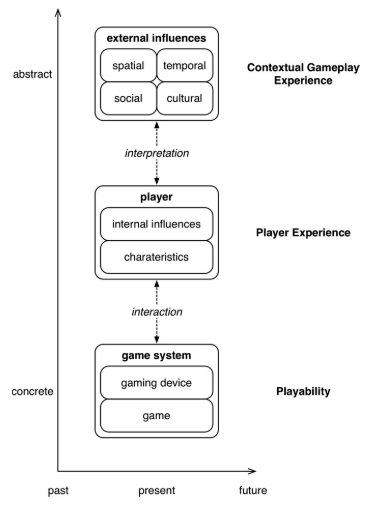
\includegraphics[width=.6\linewidth]{gfx/ref_framework/context_gp_exp}} \quad
\caption[The Contextual Gameplay Experience Model]{The Contextual Gameplay Experience Model \autocite{Engl2013}}\label{fig:context_gp_exp}
\end{figure}

%----------------------
\subsection{Playability}
\label{sec:playability}
\textcite{Sanchez2012} proposed playability as a qualitative measurement of the quality of a digital game, comprising hedonic and pragmatical aspects of \ac{PX}. As expected, the authors argue that \ac{PX} should be evaluated regarding different points of views, which they call facets. They identified the following six facets:

\begin{enumerate}
    \item \emph{Intrinsic playability}: it comprises all the elements which are inherent to the nature of a digital game; e.g., gameplay design and mechanics.
    \item \emph{Mechanical playability}: it represents the quality of a digital game as a software system. It comprises aspects like the game engine, frame rate and lighting.
    \item \emph{Interactive playability}: it represents the interaction between a player and a digital game. It is mainly related to the game \ac{UI}.
    \item \emph{Artistic playability}: it is related to the artistic aspects and aesthetics of a digital game.
    \item \emph{Personal playability}: it represents the individual actions and feelings of a player when playing a digital game.
    \item \emph{Interpersonal playability}: it represents the perceptions and feelings of players when playing as a group.
\end{enumerate}

The playability (including each facet) of a digital game is measured by assessing the following attributes:

\begin{itemize}
    \item \emph{Satisfaction}: it is the gratification derived from playing a digital game. The authors propose to measure these attribute using other aspects; i.e., fun, disappointment and attractiveness.
    \item \emph{Learnability}: it is the understanding and mastery of a player regarding the game system and mechanics. This attribute includes game knowledge, skill, difficulty, frustration, speed and discovery.
    \item \emph{Effectiveness}: it includes the time and resources necessary to provide players with an entertaining experience. This attribute is measured through completion and structuring (i.e., when, where and how game elements appear in a game).
    \item \emph{Immersion}: it represents the degree of realism to which a player feels involved in a game world. This attribute comprises conscious awareness, absorption, realism and dexterity.
    \item \emph{Motivation}: it includes the game characteristics that prompt players to complete game goals. It is measured through encouragement, curiosity, self-improvement and diversity.
    \item \emph{Emotion}: it represents the players' involuntary response to a digital game. This attribute is measured through reaction, conduct and sensory appeal.
    \item \emph{Socialisation}: it represents the game elements that promote social experiences. This attribute comprises social perception, group awareness, personal implication, sharing, communication and interaction.
\end{itemize}

To measure playability, evaluators can use different \ac{GUR} methods, such as game metrics, questionnaires, interviews and heuristics inspection. They should identify metrics (e.g. experts' rates in a heuristic evaluation) to measure each attribute. The overall playability of a digital game is the total sum of values across all attributes in the different facets.
%----------------------
\subsection{A Physiological Evaluation Model for Flow-Experience in VR Games: Construction and Preliminary Test}

\textcite{Bian2015} present a physiological model for evaluating flow experience in virtual reality games. Flow is a state in which players are fully immersed and engaged in a game.

Flow is mainly evaluated using self-report questionnaires, which collect data from players after interaction. This evaluation have two main limitations: (i) collected evaluation data is subjective and (ii) data collection occurs when players are not in flow state anymore.

The proposed model addresses these two issues using physiological flow indicators which are measured during interaction. The model includes 5 first level indicators, which are: \ac{EMG}, cardiovascular activity, \ac{EDA}, respiratory activity and \ac{EEG}.

After conducting an empirical study, obtained results revealed that heart rate, inter beat interval, heart rate variability, low-frequency band, high frequency band heart rate variability, and respiratory rate predict flow experience effectively.

%----------------------
\subsection{User Satisfaction Evaluation Model Based on Blink Interval}

\textcite{hou2015} present a user satisfaction evaluation model based on blink interval. The model is intended to overcome weaknesses of usability methods like self-report questionnaires providing and objective evaluation model. These weaknesses include: users tend to choose what is socially desirable, they may get confused about definitions of scales and they may get bored when answering long questionnaires, consequently the tend to provide random answers.

The authors found that blink interval may a be an effective physiological indicator of user satisfaction. They identified a strong correlation between user's blink interval and their satisfaction when using a system. The results showed that the lower the satisfaction is, the longer the blink interval is. To validate the model an eye tracker was employed. 31 participants were asked to perform two tasks: shop online and tag on a micro blog.

The limitations of the model are related to the impact that environment could have on blink interval. Also, authors remark that the model would be more appropriate for identifying user dissatisfaction.

